% -----------------------------------------------------------------------------
%
% Copyright (c) 2017 Sam Cox, Roberto Sommariva
%
% This file is part of the AtChem2 software package.
%
% This file is covered by the MIT license which can be found in the file
% LICENSE.md at the top level of the AtChem2 distribution.
%
% -----------------------------------------------------------------------------

\chapter{Introduction} \label{ch:introduction}

\textbf{AtChem2} is an open source modelling tool for atmospheric
chemistry. It is designed to build and run zero-dimensional
box-models using the Master Chemical Mechanism
(\href{https://mcm.york.ac.uk/MCM}{MCM}). The \textbf{MCM} is a
near-explicit chemical mechanism which describes the gas-phase
oxidation of primary emitted Volatile Organic Compounds (VOC) to
carbon dioxide (\cf{CO2}) and water (\cf{H2O}). The MCM protocol is
detailed in \citet{jenkin_1997} and subsequent updates
\citep{saunders_2003, jenkin_2003, bloss_2005, jenkin_2012, jenkin_2015}.
Although it is meant to be used with the MCM, AtChem2 can use any
other chemical mechanism, as long as it is in the correct format
(Sect.~\ref{sec:chemical-mechanism}).

AtChem2 is a development of \textbf{AtChem-online}, a modelling web
tool created at the University of Leeds to facilitate the use of the
MCM in the simulation of laboratory and environmental chamber
experiments within the \href{https://www.eurochamp.org}{EUROCHAMP}
community \citep{martin_2009}. AtChem-online runs as a
\href{https://atchem.york.ac.uk}{web service}, provided by the
University of York: in order to use AtChem-online, the user needs only
a text editor, a file compression tool, a web browser, and an internet
connection. A tutorial -- with examples and exercises -- is available on
the \href{https://mcm.york.ac.uk/MCM/atchemonline/intro}{MCM website}.

AtChem-online is easy to use even for inexperienced users but has a
number of limitations, mostly related to its nature as a web
application. \textbf{AtChem2} was developed from AtChem-online; the
aim is to provide an \emph{offline} modelling tool capable of running
long simulations of computationally intensive models, as well as batch
simulations for sensitivity studies. In addition, AtChem2 implements a
continuous integration workflow, coupled with a comprehensive
Testsuite and version control (\href{https://git-scm.com}{git}) which
makes it robust, reliable and traceable.

The codebase of AtChem2 is structured into four components (or layers)
-- as illustrated in Fig.~\ref{fig:atchem-arch} -- and is written
mostly in Fortran 90/95. Installation, compilation and execution of
AtChem2 are semi-automated via a number of shell and Python scripts
that require minimal input from the user. This document
(\texttt{AtChem2-Manual.pdf}) is the AtChem2 user manual and contains
all the information required to install, configure, and use the
current version of AtChem2. A summary of these instructions with
additional information, and a list of \underline{known issues} can be
found on the \href{https://github.com/AtChem/AtChem2/wiki}{wiki}.

\begin{figure}[htb]
  \centering
  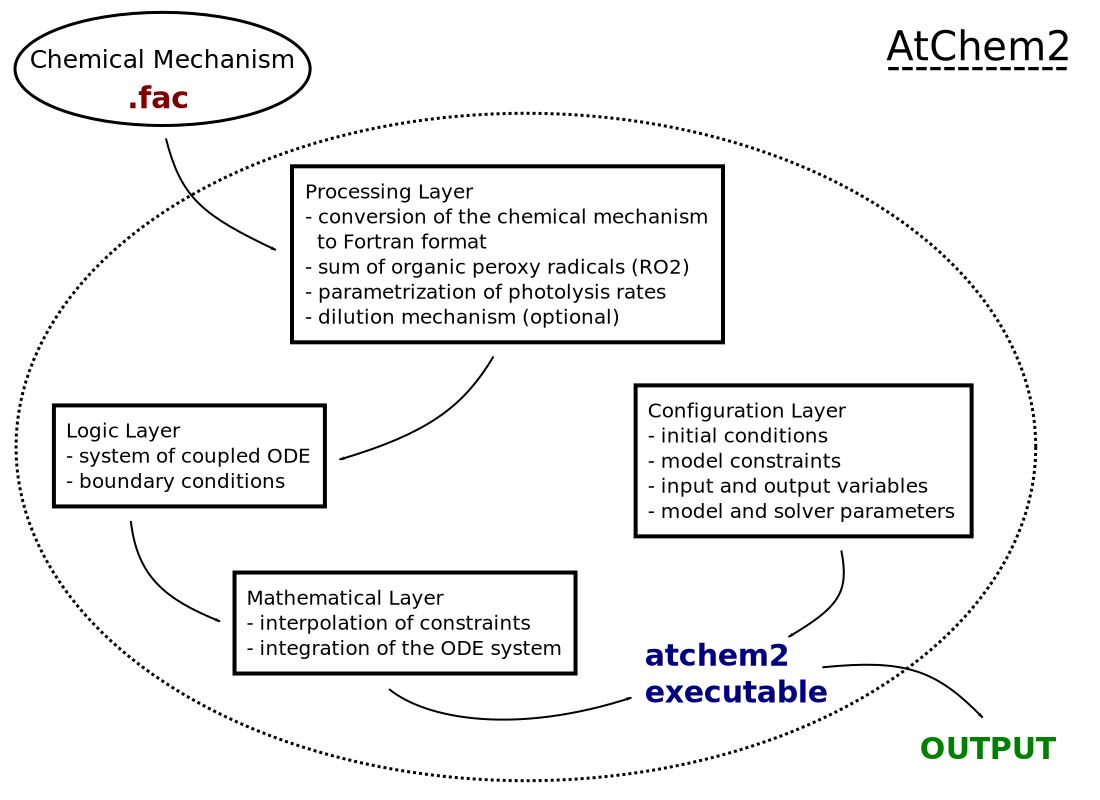
\includegraphics[width=0.8\textwidth]{atchem-structure.png}
  \caption{Architecture of AtChem2.}
  \label{fig:atchem-arch}
\end{figure}

% -------------------------------------------------------------------- %
\section{Conventions} \label{sec:conventions}

The following conventions are adopted in the AtChem2 user manual and
documentation:

\begin{description}
\item[\maindir] is the base directory of the AtChem2 model.\\
  For example: \texttt{\$HOME/AtChem2/}.
\item[\depdir] is the directory where the AtChem2 dependencies are installed.\\
  For example: \texttt{\$HOME/AtChem-lib/}.
\item[\sharedir] is the directory for the pre-compiled chemical
  mechanism shared library (\texttt{mechanism.so}).\\
  By default, it is \texttt{model/configuration/} inside the \maindir.
\end{description}

The user can change the locations and names of these directories
according to their setup, workflow, personal preferences, etc\ldots As
long as the correct paths to the libraries and directories needed by
AtChem2 are specified, the model will compile and run.\\

\textcolor{red}{\bf Important Note}: AtChem2 runs in
\textbf{Coordinated Universal Time (UTC)}, with no daylight
saving. This is to simplify the calculation of the solar angles and,
therefore, of the photolysis rates. The user must ensure that the
input data and the model constraints are provided in UTC (i.e. GMT
timezone) and convert the output to Local Time, if needed.

% -------------------------------------------------------------------- %
\section{License and citation} \label{sec:license-citation}

AtChem2 is open source and free to use, under the terms of the
\textbf{MIT license}. A copy of the license can be found in the
\texttt{LICENSE} file. If used in a publication, please cite the GMD
paper \citep{sommariva_2020}:\\

R.~Sommariva, S.~Cox, C.~Martin, K.~Boro{\'n}ska, J.~Young, P.~K. Jimack,
M.~J. Pilling, V.~N. Matthaios, B.~S. Nelson, M.~J. Newland, M.~Panagi,
W.~J. Bloss, P.~S. Monks, and A.~R. Rickard.
\textbf{AtChem (version 1), an open-source box model for the Master Chemical Mechanism}.
\textit{Geoscientific Model Development}, 13, 1, 169--183, 2020.
doi: \href{https://doi.org/10.5194/gmd-13-169-2020}{10.5194/gmd-13-169-2020}.
